% SPDX-License-Identifier: Apache-2.0
% Native manuscript source. Build from the repository root with make paper.
\documentclass{article}
\usepackage[T1]{fontenc}
\usepackage[utf8]{inputenc}
\input{glyphtounicode}
\pdfgentounicode=1
% Computer Modern's sized brackets need explicit text-extraction mappings.
\pdfglyphtounicode{bracketleftbig}{005B}
\pdfglyphtounicode{bracketrightbig}{005D}
\pdfglyphtounicode{bracketleftBig}{005B}
\pdfglyphtounicode{bracketrightBig}{005D}
\pdfglyphtounicode{bracketleftbigg}{005B}
\pdfglyphtounicode{bracketrightbigg}{005D}
\pdfglyphtounicode{bracketleftBigg}{005B}
\pdfglyphtounicode{bracketrightBigg}{005D}
\usepackage{microtype}
\usepackage{graphicx}
\usepackage{booktabs,tabularx}
\usepackage{amsmath,amssymb,amsthm,mathtools}
\usepackage{siunitx}
\usepackage{enumitem}
\usepackage{tikz}
\usetikzlibrary{arrows.meta,calc,positioning,patterns,fit}
\usepackage{pgfplots}
\pgfplotsset{compat=1.18}
\usepackage{subcaption}
\usepackage{xurl}
\usepackage[hyperfootnotes=false]{hyperref}
\usepackage[preprint]{icml2026}
\usepackage[capitalize,noabbrev]{cleveref}

% The supplied author has no stated institutional affiliation or contact email.
% Retain the preprint notice and use the repository as the artifact contact.
\makeatletter
\renewcommand{\printAffiliationsAndNotice}[1]{%
  \global\icml@noticeprintedtrue
  {\let\thefootnote\relax\footnotetext{\hspace*{-\footnotesep}%
    \href{https://github.com/SamMausberg/contracted-moment-kernels}{Code, proofs, and measurements.}\\
    \Notice@String}}}
\makeatother

\definecolor{cmkblue}{HTML}{2369A1}
\definecolor{cmkorange}{HTML}{CC6534}
\definecolor{cmkgreen}{HTML}{208578}
\definecolor{cmkgray}{HTML}{71808D}
\hypersetup{pdftitle={When Moment Summaries Can Certify Attention},
  pdfauthor={Sam Mausberg},pdfsubject={Research preprint: attention certificates and GH200 experiments},colorlinks=true,
  linkcolor=cmkblue,citecolor=cmkblue,urlcolor=cmkblue}
\sisetup{detect-all,group-separator={,},group-minimum-digits=4}
\newtheorem{theorem}{Theorem}[section]
\newtheorem{lemma}[theorem]{Lemma}
\newtheorem{proposition}[theorem]{Proposition}
\newtheorem{corollary}[theorem]{Corollary}
\theoremstyle{definition}
\newtheorem{definition}[theorem]{Definition}
\newtheorem{example}[theorem]{Example}
\theoremstyle{remark}
\newtheorem{remark}[theorem]{Remark}
\DeclareMathOperator{\diag}{diag}
\newcommand{\R}{\mathbb{R}}
\DeclarePairedDelimiter{\abs}{\lvert}{\rvert}
\DeclarePairedDelimiter{\norm}{\lVert}{\rVert}
\newcommand{\ip}[2]{\langle #1,#2\rangle}
\newcommand{\code}[1]{\texttt{\detokenize{#1}}}
\newcommand{\artifact}[2]{\href{https://github.com/SamMausberg/contracted-moment-kernels/blob/main/#1}{#2}}
\icmltitlerunning{When Moment Summaries Can Certify Attention}

\begin{document}
\twocolumn[
\icmltitle{When Moment Summaries Can Certify Attention}
\begin{icmlauthorlist}
\icmlauthor{Sam Mausberg}{}
\end{icmlauthorlist}
\icmlkeywords{attention, verified numerics, moment methods, Lean, GPU kernels}
\vskip 0.3in
]
\printAffiliationsAndNotice{}

\begin{abstract}
Moment summaries can avoid a token scan if their uncertainty cannot change
the required output decision.
We characterize this condition exactly for independent block intervals,
derive exponential-attention bounds from projected signed moments,
and tighten them using dependence between block mass and value range.
A Lean development proves the real-arithmetic certificate chain;
all 64 theorems build and pass an axiom audit.
Exact-rational experiments certify 61 of 149 coordinates with value coupling
versus 57 with boxes, including one controlled gain beyond a global value hull.
On a GH200, parallel block reduction reduces a favorable screening stage from
118.65 to \SI{20.09}{\micro\second}, but the complete path remains slower than
fused dense attention; trained-model traces yield no passes in 2,016 rank-eight
head instances.
These results identify two obstacles to useful certification: exponential
bound inflation and decision/fallback overhead.
\end{abstract}

\section{Introduction}
\label{sec:introduction}

An approximate attention value and a certified output decision solve different
problems. A small absolute error can still cross a rounding boundary, while
a coarse value estimate may determine a broad downstream decision exactly.
The relevant quantity is therefore the uncertainty relative to the consumer's
decision boundary.

We study positive normalized reductions represented by block masses and
centered value moments. At any boundary $c$, the normalized comparison reduces
to the sign of an unnormalized residual $N-cZ$. Independent interval metadata
gives attained extrema of this residual. If total mass is positive throughout
the box, two strict sign tests are necessary and sufficient for every compatible
output to lie in a given open cell. A rejection identifies information missing from the box;
it need not identify an inaccurate candidate value.

We test which dependence information enables certification, which error term
prevents it on trained activations, and whether avoided token work repays
construction, screening, and fallback. The evidence combines value-coupled
bounds, a formal real-attention proof chain, and GH200 implementation ablations.

Value coupling adds certificates, although a global value hull explains most
gains. Trained activations expose discarded-score uncertainty and full-rank
Taylor inflation. Parallel reduction removes a GPU bottleneck, yet the
complete path remains slower than fused dense attention throughout the sweep.

\paragraph{Scope.}
Lean proves the real-arithmetic chain under concrete centering, radius,
symmetry, and row-sum witnesses. The rational checker and the directed CUDA
checker are tested implementations, not extracted proofs. Ordinary
NumPy/CUDA summaries do not provide outward intervals. Exact-real rounding
also differs from the accumulation contract of a particular fused GPU kernel.
\Cref{app:formalization} maps these claims to the checked theorems and remaining
implementation bridges. Code, measurements, and reproduction commands are
available in the \href{https://github.com/SamMausberg/contracted-moment-kernels}{research repository}.

\paragraph{Related work.}
Adaptive predicates refine uncertain signs \citep{shewchuk}, while Taylor
models retain polynomial structure with bounded remainders \citep{berz}.
Multipole attention combines grouped interactions and selected exact work
\citep{multipole,fma}; TaylorShift and symmetry-aware features reorganize
polynomial attention \citep{taylorshift,sata}. COBS uses covariance statistics
for block selection, SPLA combines sparse and residual linear paths, and
LOCKS studies limits of moment summaries for broad scores
\citep{cobs,spla,locks}. WitCert and attention-memory observability contracts
already connect runtime witnesses, formal scope, and fallback
\citep{observability,witcert}. Our focus is the consumer-specific residual
interface, the projected signed moments supplying it, and stronger mass/value
dependence. These general principles are established; comparisons with
unreproduced systems concern method scope, not measured performance.

\section{Certificates at Observation Boundaries}
\label{sec:certificates}

Partition a finite, nonempty visible input into nonempty blocks
$b=1,\ldots,B$. A positive normalized reduction has coordinates
\begin{equation}
 y_j=N_j/Z,\quad N_j=\sum_b n_{bj},\quad Z=\sum_b z_b>0.
 \label{eq:normalized-reduction}
\end{equation}
For fixed centers $\nu_{bj}$, write $m_{bj}=n_{bj}-\nu_{bj}z_b$ and assume
sound metadata
\begin{equation}
 0\le l_b\le z_b\le u_b,\qquad
 m^-_{bj}\le m_{bj}\le m^+_{bj}.
 \label{eq:block-boxes}
\end{equation}
All quantities must describe the same input, mask, query, scaling, and data
version. Positivity of $Z$ is a separate premise; $\sum_b l_b>0$ suffices.

An \emph{observation cell} $(a_j,b_j)$ is an open interval on which the consumer
is constant. Proving $y_j$ belongs to this cell therefore determines its
observation. For finite numerical BF16 rounding, neighboring representable
values supply midpoint boundaries; strict containment avoids ties. This
contract does not distinguish positive and negative zero by their bits.
Alternatively, a monotone consumer $Q$ satisfies $Q(l)=Q(u)\Rightarrow
Q(y)=Q(l)$ whenever $l\le y\le u$. A concrete IEEE-754 model and its
monotonicity theorem are not supplied.

\subsection{Exact Certificates for Independent Boxes}

At a boundary $c$, define
\begin{equation}
 \begin{split}
 \mathcal L_j(c)&=\sum_b m^-_{bj}\\
 &\quad+\sum_b\min\{(\nu_{bj}-c)l_b,(\nu_{bj}-c)u_b\},
 \end{split}
 \label{eq:lower-residual}
\end{equation}
\begin{equation}
 \begin{split}
 \mathcal U_j(c)&=\sum_b m^+_{bj}\\
 &\quad+\sum_b\max\{(\nu_{bj}-c)l_b,(\nu_{bj}-c)u_b\}.
 \end{split}
 \label{eq:upper-residual}
\end{equation}

\begin{theorem}[Boundary certificate]\label{thm:boundary-certificate}
Under \cref{eq:normalized-reduction,eq:block-boxes},
\begin{equation}
 \mathcal L_j(c)\le N_j-cZ\le\mathcal U_j(c).
 \label{eq:residual-enclosure}
\end{equation}
Consequently,
\begin{equation}
 \begin{gathered}
 \mathcal L_j(a_j)>0,\qquad \mathcal U_j(b_j)<0\\
 \Longrightarrow\quad a_j<y_j<b_j.
 \end{gathered}
 \label{eq:cell-certificate}
\end{equation}
\end{theorem}
\begin{proof}
The centered residual identity is
\begin{equation}
 N_j-cZ=\sum_b\bigl[m_{bj}+(\nu_{bj}-c)z_b\bigr].
 \label{eq:residual-identity}
\end{equation}
For any scalar $\alpha$, the extrema of $\alpha z$ on $[l,u]$ are
$\min(\alpha l,\alpha u)$ and $\max(\alpha l,\alpha u)$. Apply these bounds
to each summand and sum. Dividing the strict residual signs by $Z>0$ gives
the cell inequalities.
\end{proof}

The certificate requires no division. A numerical quotient may choose a
candidate cell: a poor choice reduces acceptance but cannot invalidate sound
residual signs.

\begin{theorem}[Optimality for independent metadata]\label{thm:box-optimality}
Over the Cartesian product of the intervals in \cref{eq:block-boxes},
$\mathcal L_j(c)$ and $\mathcal U_j(c)$ are the attained minimum and maximum
of the residual at each fixed $c$.
\end{theorem}
The proof is given in \cref{app:box-optimality}.

This optimality concerns the stated product box. Actual masses and numerators
can be correlated, and the two extrema need not come from the same input.
Residual optimality needs no positive lower bound on total mass; interpreting
every extremizer as a normalized output additionally requires $\sum_b l_b>0$.

\begin{corollary}[Sufficiency of box metadata]\label{cor:box-sufficiency}
If $\sum_b l_b>0$, every compatible box output belongs to $(a_j,b_j)$ if and
only if $\mathcal L_j(a_j)>0$ and $\mathcal U_j(b_j)<0$.
\end{corollary}
\begin{proof}
Sufficiency follows from \cref{thm:boundary-certificate}. If the lower test
fails, \cref{thm:box-optimality} supplies a vertex with residual at $a_j$ at
most zero. Its denominator is positive, so its output is at most $a_j$.
The upper extremizer gives the corresponding counterexample at $b_j$.
\end{proof}

A rejection thus means that the metadata admits a conflicting output, even
if the original tokens cannot realize that vertex. Acceptance then needs
tighter bounds, retained dependence, or a different observation contract.

The two-block example in \cref{ex:boundary-geometry,fig:boundary-geometry}
shows a strict improvement over a symmetric midpoint residual bound.

\subsection{Refinement and Retained Value Dependence}

\begin{theorem}[Monotone refinement]\label{thm:refinement}
Replacing each interval by a nonempty subinterval cannot decrease
$\mathcal L_j(c)$ or increase $\mathcal U_j(c)$ at a fixed boundary $c$.
Intersecting two sound enclosures preserves the truth.
\end{theorem}
\begin{proof}
A minimum over a smaller feasible set cannot decrease, and a maximum cannot
increase. Apply this fact to every block and sum. A point contained in both
enclosures belongs to their intersection.
\end{proof}

Selected blocks may therefore be refined without discarding earlier work.
The invariant is sound enclosure; the implementation's uncertainty priority
is a heuristic. Monotonicity applies to a fixed cell. Refinement need not
terminate with a strict certificate at a rounding midpoint, so execution
requires bounded work and a tie-aware path or declared reference fallback.

For nonnegative block weights, exact centered value extrema
$p_{bj}=\min_{i\in b}(v_{ij}-\nu_{bj})$ and
$q_{bj}=\max_{i\in b}(v_{ij}-\nu_{bj})$ imply
\begin{equation}
 p_{bj}z_b\le m_{bj}\le q_{bj}z_b:
 \label{eq:value-coupling}
\end{equation}
multiply each value inequality by its weight and sum. Retain this dependence
by defining the nonempty compact polygon
\begin{equation}
 P_{bj}=\left\{(z,m):\begin{aligned}
 &l_b\le z\le u_b,\\
 &m^-_{bj}\le m\le m^+_{bj},\\
 &p_{bj}z\le m\le q_{bj}z
 \end{aligned}\right\}.
 \label{eq:coupled-polygon}
\end{equation}

\begin{theorem}[Coupled certificate]\label{thm:coupled-certificate}
In \cref{eq:lower-residual,eq:upper-residual}, replace each block term by the
minimum or maximum, respectively, of $m+(\nu_{bj}-c)z$ over $P_{bj}$.
The resulting residual enclosure and cell certificate are sound, never wider
than the box bounds, and improve monotonically under sound box intersection
with fixed value extrema.
\end{theorem}
\begin{proof}
The true pair belongs to $P_{bj}$ by \cref{eq:block-boxes,eq:value-coupling}.
The residual identity remains unchanged. Each polygon is contained in its
rectangle, and shrinking the rectangle shrinks its intersection with the
fixed cone. The extrema can only improve; summation and $Z>0$ finish the proof.
\end{proof}

The rational optimizer evaluates these extrema at polygon vertices using a
constant number of rational operations per block/channel; bit cost depends
on the fractions. The complete enumeration argument is in
\cref{app:polygon-support}. Inconsistent metadata is rejected.

Joint optimization can be strictly tighter than intersecting separate scalar
bounds; \cref{ex:joint-coupling} gives an exact example.

\begin{figure*}[!t]
 \centering
 % Native vector fragment. Required: tikz; arrows.meta; cmk{blue,orange,green,gray}.
% Exact polygon: (1,-1/4),(3,-3/4),(3,3/2),(1,1/2).
% Right-panel residuals are M+(1-c)Z; all endpoints are exact terminating decimals.
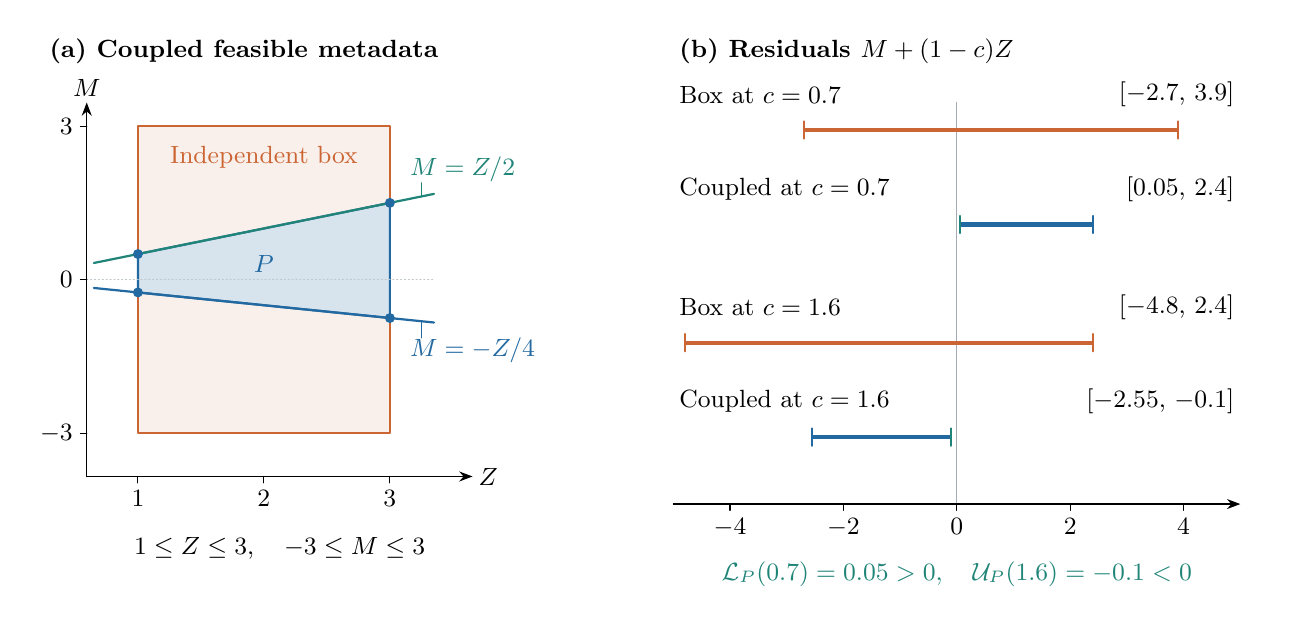
\begin{tikzpicture}[font=\small, line cap=round, line join=round,
  >=Stealth, every node/.style={inner sep=2pt}]
  \path[use as bounding box] (-0.2,-0.65) rectangle (15.7,6.6);
  \node[anchor=west,font=\small\bfseries] at (0,6.3)
    {(a) Coupled feasible metadata};
  % x = 1.2 + 1.6(Z-1); y = 3.4 + 0.65M.
  \filldraw[fill=cmkorange!10,draw=cmkorange,thick]
    (1.2,1.45) rectangle (4.4,5.35);
  \node[text=cmkorange] at (2.8,4.95) {Independent box};
  \filldraw[fill=cmkblue!18,draw=cmkblue,thick]
    (1.2,3.2375)--(4.4,2.9125)--(4.4,4.375)--(1.2,3.725)--cycle;
  \draw[cmkgray!45,thin,densely dotted] (0.55,3.4)--(4.96,3.4);
  \draw[cmkblue,thick] (0.64,3.294375)--(4.96,2.855625);
  \draw[cmkgreen,thick] (0.64,3.61125)--(4.96,4.48875);
  \node[text=cmkblue] at (2.8,3.6) {$P$};
  \node[anchor=west,text=cmkgreen,font=\small] at (4.58,4.8)
    {$M=Z/2$};
  \draw[cmkgreen,thin] (4.8,4.63)--(4.8,4.45625);
  \node[anchor=west,text=cmkblue,font=\small] at (4.58,2.5)
    {$M=-Z/4$};
  \draw[cmkblue,thin] (4.8,2.66)--(4.8,2.871875);
  \foreach \x/\y in {1.2/3.2375,4.4/2.9125,4.4/4.375,1.2/3.725}
    \fill[cmkblue] (\x,\y) circle (1.8pt);
  \draw[->] (0.55,0.9)--(5.45,0.9) node[anchor=west] {$Z$};
  \draw[->] (0.55,0.9)--(0.55,5.65) node[anchor=south] {$M$};
  \foreach \x/\lab in {1.2/1,2.8/2,4.4/3} {
    \draw (\x,0.9)--(\x,0.82);
    \node[anchor=north,font=\small] at (\x,0.8) {$\lab$};
  }
  \foreach \y/\lab in {1.45/-3,3.4/0,5.35/3} {
    \draw (0.55,\y)--(0.47,\y);
    \node[anchor=east,font=\small] at (0.45,\y) {$\lab$};
  }
  \node[anchor=north,font=\small] at (3,0.2)
    {$1\leq Z\leq3,\quad -3\leq M\leq3$};
  \begin{scope}[xshift=8cm]
    \node[anchor=west,font=\small\bfseries] at (0,6.3)
      {(b) Residuals $M+(1-c)Z$};
    % x = 0.72(residual+5). The zero line separates the sign tests.
    \draw[cmkgray!65,thin] (3.6,0.55)--(3.6,5.65);
    \node[anchor=west,font=\small] at (0,5.75)
      {Box at $c=0.7$};
    \node[anchor=east,font=\small] at (7.2,5.75)
      {$[-2.7,\,3.9]$};
    \draw[cmkorange,line width=1.5pt,line cap=butt] (1.656,5.3)--(6.408,5.3);
    \foreach \x in {1.656,6.408}
      \draw[cmkorange,line width=0.7pt] (\x,5.19)--(\x,5.41);
    \node[anchor=west,font=\small] at (0,4.55) {Coupled at $c=0.7$};
    \node[anchor=east,font=\small] at (7.2,4.55)
      {$[0.05,\,2.4]$};
    % A round endpoint marker would straddle zero at the exact +0.05 bound.
    % Thin terminal caps preserve the visible strict sign at this scale.
    \draw[cmkblue,line width=1.5pt,line cap=butt] (3.636,4.1)--(5.328,4.1);
    \draw[cmkgreen,line width=0.7pt] (3.636,3.99)--(3.636,4.21);
    \draw[cmkblue,line width=0.7pt] (5.328,3.99)--(5.328,4.21);
    \node[anchor=west,font=\small] at (0,3.05)
      {Box at $c=1.6$};
    \node[anchor=east,font=\small] at (7.2,3.05)
      {$[-4.8,\,2.4]$};
    \draw[cmkorange,line width=1.5pt,line cap=butt] (0.144,2.6)--(5.328,2.6);
    \foreach \x in {0.144,5.328}
      \draw[cmkorange,line width=0.7pt] (\x,2.49)--(\x,2.71);
    \node[anchor=west,font=\small] at (0,1.85) {Coupled at $c=1.6$};
    \node[anchor=east,font=\small] at (7.2,1.85)
      {$[-2.55,\,-0.1]$};
    \draw[cmkblue,line width=1.5pt,line cap=butt] (1.764,1.4)--(3.528,1.4);
    \draw[cmkblue,line width=0.7pt] (1.764,1.29)--(1.764,1.51);
    \draw[cmkgreen,line width=0.7pt] (3.528,1.29)--(3.528,1.51);
    \draw[->] (0,0.55)--(7.2,0.55);
    \foreach \x/\lab in {0.72/-4,2.16/-2,3.6/0,5.04/2,6.48/4} {
      \draw (\x,0.55)--(\x,0.47);
      \node[anchor=north,font=\small] at (\x,0.45) {$\lab$};
    }
    \node[anchor=north,font=\small,text=cmkgreen] at (3.6,-0.1)
      {$\mathcal L_P(0.7)=0.05>0,\quad\mathcal U_P(1.6)=-0.1<0$};
  \end{scope}
\end{tikzpicture}

 \caption{An analytic coupled-geometry example: value dependence removes box
 corners that obstruct both boundary signs. The target interval is illustrative.}
 \label{fig:coupled-geometry}
\end{figure*}

Lean proves the positive-weight coupling and box certificate. The polygon
optimizer has the argument in \cref{app:polygon-support} and independent exact geometry tests; its
executable correctness is not formalized.

A sufficient margin-versus-width condition explains difficult near-midpoint
coordinates and eventual certification under convergent sound refinement
(\cref{prop:margin-uncertainty}).

\section{Projected Signed-Moment Enclosures}
\label{sec:moments}

Attention has the exact-real form
\begin{equation}
 y_j(q)=\frac{\sum_i e^{q^Tk_i}v_{ij}}{\sum_i e^{q^Tk_i}}.
 \label{eq:attention}
\end{equation}
The query includes attention scaling; keys are those attended to after
positional transformations. Let $\mu_b,\nu_b$ be exact block means and set
$\delta_i=k_i-\mu_b$, $x_i=v_i-\nu_b$. Select $r\le d$ coordinates and write
\begin{equation}
 \begin{gathered}
 q^T\delta_i=t_i+e_i,\qquad t_i=u^T\delta_i^{(r)},\\
 |t_i|\le\rho_b,\qquad |e_i|\le\epsilon_b.
 \end{gathered}
 \label{eq:score-split}
\end{equation}
The implementation selects a coordinate prefix; permutation permits another
fixed subset. No approximate PCA basis is substituted. Stored coordinate
radii $a_{bk}\ge\max_{i\in b}|\delta_{ik}|$ and value radii
$R_{bj}\ge\max_{i\in b}|x_{ij}|$ give
\begin{equation}
 \rho_b=\sum_{k<r}|q_k|a_{bk},\qquad
 \epsilon_b=\sum_{k\ge r}|q_k|a_{bk}.
 \label{eq:query-radii}
\end{equation}

\subsection{Signed Moments and a Quadratic Witness}

Using block means, store
\begin{equation}
 \begin{aligned}
 \Sigma_b&=\operatorname{mean}(\delta^{(r)}\delta^{(r)T}),\\
 C_b&=\operatorname{mean}(\delta^{(r)}x^T),\\
 H_{bj}&=\operatorname{mean}(\delta^{(r)}\delta^{(r)T}x_j).
 \end{aligned}
 \label{eq:stored-moments}
\end{equation}
The full signed tensor $H$ is temporary construction data. Query metadata
retains its diagonal $D_{bj}$ and a witness
\begin{equation}
 \eta_{bj}\ge\max_a\sum_k|(H_{bj}-D_{bj})_{ak}|.
 \label{eq:rowsum-witness}
\end{equation}
Here $D$ denotes either the diagonal matrix or its stored diagonal. Choosing
$D=0$ is also valid. For $r=0$, the empty row-sum witness is zero.

\begin{lemma}[Quadratic witness]\label{lem:quadratic-witness}
If $F$ is symmetric and $\eta\ge\max_a\sum_k|F_{ak}|$, then
$|u^TFu|\le\eta\|u\|_2^2$.
\end{lemma}
The proof is given in \cref{app:quadratic-witness}.

Retaining the diagonal weakly reduces the row-sum witness but shifts the center;
intervals need not be nested or improve acceptance
(\cref{app:diagonal-nonnesting}).

\subsection{A Sharp Exponential Remainder}

Define the nonnegative coefficient
\begin{equation}
 \kappa(\rho)=
 \begin{cases}
 (e^\rho-1-\rho-\rho^2/2)/\rho^2,&\rho>0,\\
 0,&\rho=0.
 \end{cases}
 \label{eq:kappa}
\end{equation}
\begin{lemma}[Sharp quadratic majorant]\label{lem:sharp-remainder}
For $\rho\ge0$ and $|t|\le\rho$,
\begin{equation}
 \begin{gathered}
 |e^t-1-t-t^2/2|\le\kappa(\rho)t^2,\\
 \kappa(\rho)\le e^\rho\rho/6.
 \end{gathered}
 \label{eq:sharp-remainder}
\end{equation}
For $\rho>0$, the second inequality is strict and $\kappa(\rho)$ is the
smallest uniform quadratic coefficient on $[-\rho,\rho]$.
\end{lemma}
The proof is given in \cref{app:sharp-remainder}.

At radius zero, zero is the chosen nonnegative coefficient; minimality over
arbitrary real coefficients is not claimed. Near zero, numerical evaluation
uses a series to avoid cancellation. It is not outward without a bounded
remainder; the rational path instead uses an upper enclosure of $e^\rho$.
Lean derives the bound from the convergent real exponential series and
discharges the remainder premise of the subsequent lifting lemma.

The remainder and discarded-score inflation retain exponential growth
(\cref{fig:remainder-mechanism}).

\subsection{From Moments to Full-Score Blocks}

Choose any common finite shift $s$ and define the actual quantities
\begin{equation}
 \begin{aligned}
 z_b(s)&=\sum_{i\in b}e^{q^Tk_i-s},\\
 m_{bj}(s)&=\sum_{i\in b}e^{q^Tk_i-s}x_{ij}.
 \end{aligned}
 \label{eq:shifted-blocks}
\end{equation}
The factor $e^{-s}$ cancels from \cref{eq:attention}; all following bounds and
residuals concern these shifted quantities. Set
\begin{equation}
 \begin{aligned}
 a_b&=q^T\mu_b, & w_b&=n_b e^{a_b-s},\\
 \sigma_b^2&=u^T\Sigma_bu, & A_b&=1+\sigma_b^2/2,\\
 \tau_b&=\kappa(\rho_b)\sigma_b^2.
 \end{aligned}
 \label{eq:moment-scalars}
\end{equation}
\begin{equation}
 \begin{aligned}
 \widetilde l_b&=w_b\max\{1,A_b-\tau_b\},\\
 \widetilde u_b&=w_b(A_b+\tau_b),
 \end{aligned}
 \label{eq:projected-mass}
\end{equation}
\begin{equation}
 \begin{aligned}
 \widehat m_{bj}&=w_b\left[(C_b^Tu)_j+\tfrac12u^TD_{bj}u\right],\\
 \beta_{bj}&=w_b\left[\tfrac12\eta_{bj}\|u\|_2^2+\tau_bR_{bj}\right].
 \end{aligned}
 \label{eq:projected-numerator}
\end{equation}
Here $n_b$ is the block cardinality.

\begin{samepage}
\begin{theorem}[Full-score block enclosures]\label{thm:full-score-enclosures}
Under the centering, radius, symmetry, and row-sum conditions above, sound
bounds for \cref{eq:shifted-blocks} are
\begin{gather}
 l_b=e^{-\epsilon_b}\widetilde l_b,\qquad
 u_b=e^{\epsilon_b}\widetilde u_b,\label{eq:full-mass}\\
 m^\pm_{bj}=\widehat m_{bj}\pm\left[\beta_{bj}+(e^{\epsilon_b}-1)\widetilde u_bR_{bj}\right].
 \label{eq:full-numerator}
\end{gather}
\end{theorem}
\end{samepage}
The proof is given in \cref{app:full-score-enclosures}.

Combining \cref{thm:full-score-enclosures,thm:boundary-certificate} certifies
the original finite per-token quotient. The Lean witness supplies centering,
radii, symmetry, and row sums; it does not assume the Taylor remainder or
output enclosure. Lean uses unnormalized finite-sum tensors: multiply this
paper's $H,D,\eta$ by $n_b$ to obtain that representation. Matching the score
decomposition and partition to the caller's data remains necessary; the
theorem is not a Python summary validator.

Both endpoint ranks are included. At $r=0$, retained centered moments vanish
and all score variation is discarded; at $r=d$, $\epsilon_b=0$ eliminates
projection inflation. No fixed rank is assumed useful on arbitrary trained
activations.

\subsection{Rational Evaluation and Outward Export}
\label{sec:rational-checking}

The rational implementation uses exact fractions and bounded exponential
series. For $0\le x\le1/2$, a partial sum through degree $n$ has first omitted
term $a_{n+1}=x^{n+1}/(n+1)!$. Subsequent term ratios are bounded by
$q=x/(n+2)<1$, so the tail is at most $a_{n+1}/(1-q)$.
The partial sum and that sum plus the tail enclose $e^x$. Positive interval
squaring handles range reduction; reciprocal intervals handle negative
arguments. Unsupported inputs are rejected. A separate rational
exponential-sum oracle uses no moment formulas; refinement intersects its
result with the existing enclosure. These expensive routines are correctness
artifacts, not the proposed fast GPU implementation.

Export converts rational endpoints outward to binary64 and compares each
float's exact rational value with its source. Centers also receive intervals
because rational means may be unrepresentable. The host checker expands basic
operations by one ULP; the CUDA draft uses directed rounding. Their validity
still requires the stated floating-point semantics and faithful compilation.
Both have been compiled and run on GH200, including memory checking of the
imported CUDA path; neither is extracted from Lean. Ordinary NumPy/CUDA
moment estimates do not become sound metadata through directed rounding of
the final residual sum. Sound inputs remain a premise.

\section{Representation and Execution Cost}
\label{sec:execution}

For $B$ blocks, key dimension $d$, value dimension $h$, and retained rank $r$,
the base representation stores
\begin{equation}
 B(2d+r^2+2rh+3h+1)
 \label{eq:storage}
\end{equation}
scalars. Coupling adds $2Bh$ value extrema. These counts exclude original K/V,
index maps, source identities, scratch, and allocations. Original K/V remains
available for fallback.

A block-scalar pass evaluates centroid scores, variance, radii, and mass
terms once per query/block. A channel pass contracts the value moments, then
a reduction tests the two boundaries. The arithmetic cost is
$O(B(d+r^2+rh+h))$, versus $\Theta(N(d+h))$ for a direct scan. The current
CPU builder scans K/V and constructs a temporary signed tensor in
$O(N(d+h+r^2h))$ work. These are word-operation counts; they omit rational bit
complexity and do not imply a speedup. Clustering would add a setup stage.

\begin{proposition}[Reuse threshold]
\label{prop:reuse}
Let setup cost be $S\geq0$, dense-query cost $D>0$, full-output pass probability
$p$, and expected screen/decision/return cost $C\geq0$. If rejection executes
the full dense path, expected cost for $R>0$ reuses is
\begin{equation}
 T(R)=S+R\bigl[C+(1-p)D\bigr].
 \label{eq:reuse}
\end{equation}
It is below $RD$ exactly when $pD>C$ and $R>S/(pD-C)$.
\end{proposition}
\begin{proof}
Subtract $RD$ and rearrange $S<R(pD-C)$.
\end{proof}

This fixed-cost model makes the role of pass probability explicit. A
heterogeneous scheduler needs its conditional costs. Our complete measured
path is already slower than dense per query, so no finite reuse count
amortizes its setup.

The executor validates the supported domain and source identity, selects a
candidate cell, tests its boundaries, and refines or falls back under a work
cap. Exact-rational refinement intersects sound intervals; numerical CUDA
correction supplies estimates. Python fingerprints bind refinement to ordered
visible K/V, query, and shift. They do not implement concurrent cache epochs
or a serving memory manager. The measured numerical kernels compare serial,
shared-scalar, and parallel block reductions; only the last changes reduction
order. The directed imported-box checker has a separate contract.

\section{Experimental Evidence}
\label{sec:experiments}

We test coupling, trained-activation uncertainty, and GPU execution separately.
\Cref{sec:experimental-validation} records arithmetic and implementation
checks, including an executable interval defect found and repaired.

\subsection{Coupling and Localized Uncertainty}
\label{sec:coupling-experiment}

Coupling accepts four more initial coordinates than the box certificate, but
the global value hull explains three of those gains
(\cref{tab:coupling-results,fig:coupling-ablation}). The exact-rational study
uses seed 962605, four retained ranks, four key spreads, narrow and broad value
channels, exact midpoint channels, and named geometry and attention witnesses.
All 53 cases, 149 initial coordinates, and sequential refinement stages are
retained in \artifact{results/certification/coupling.json}{coupling artifact}, including construction
and actual rational fallback costs.

If all values lie in one rounding cell, positivity of attention weights already
certifies the output. The remaining prescribed witness instead places keys
$-2,2$ with values $1-1/2560,1+1/2560$ in one rank-zero block and a singleton
key $-16$ with value $3$, at $q=1$. The outlier defeats the global hull, but its
small block mass lets the coupled test certify BF16 value $1$. An independent
direct rational exponential sum verifies the certificate. This witness
isolates the interaction between local value range and mass; it does not
estimate coverage on trained models.

\begin{figure*}[!t]
  \centering
  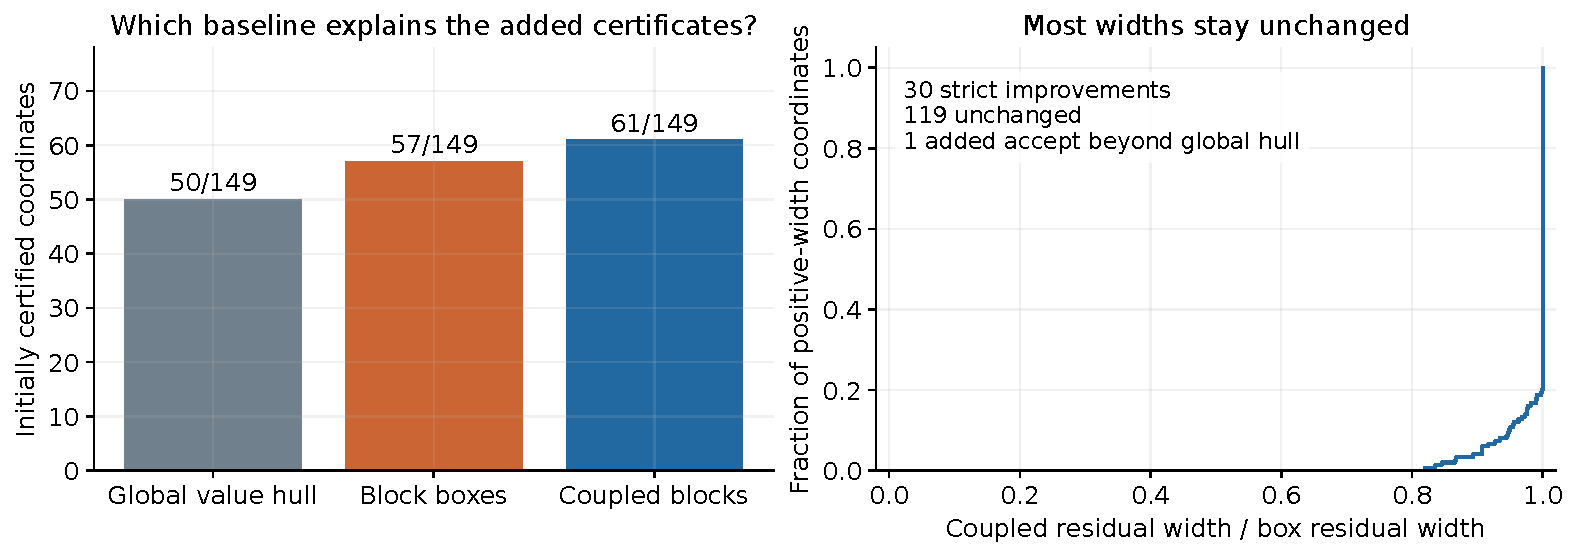
\includegraphics[width=\textwidth]{figures/coupling_ablation.pdf}
  \caption{Coupling acceptance and residual widths for all initial coordinates,
  retaining unchanged widths and refusals. The global-hull baseline explains
  most additional accepts.}
  \label{fig:coupling-ablation}
\end{figure*}

A numerical CPU experiment with $N=8192$, $d=16$, $h=8$, $B=16$, $Q=24$, and
one BLAS thread demonstrates when selective correction helps. The generator
provides favorable four-coordinate structure. Tight blocks pass all 24 queries
without correction; introducing one broad block makes every initial query fail,
but correcting that block evaluates attention weights and values for only
$1/16$ of the tokens. Broadening every block requires correcting every token
(\cref{fig:selective-refinement}). The correction-token counter excludes the
Python executor's full-source input validation and fingerprint passes, which
read K/V even without correction. CPU query times include these reads and
executed correction or fallback; construction is recorded separately.
Every complete Python path is slower than
dense NumPy: the experiment measures uncertainty localization, not GPU speed.


The GPU controls show why coordinate coverage alone is insufficient. Moderate
inputs pass 10,197 of 19,008 coordinates across repeated rank configurations,
but none of 297 complete outputs. A centered-value control passes 1,986 of
2,048 coordinates and only 6 of 32 outputs. Every coordinate must pass before
an output is accepted; any failure triggers the measured full-batch fallback.
\Cref{sec:localized-uncertainty} retains the control protocol and strict
midpoint refusals.

\subsection{Trained Post-RoPE Activations}
\label{sec:trained-activations}

Neither trained activation set produces a numerical coordinate or whole-output
pass. We capture post-RoPE Q/K/V from Qwen2.5-0.5B \citep{qwen25} on prose,
code, and arithmetic probes at prefix lengths 1,024 and 4,096. Rank eight
covers 24 layers and 14 query heads: 2,016 head instances and 129,024
coordinates. Full rank in layers 0, 12, and 23 adds 252 head instances.
\Cref{sec:trained-protocol} specifies the model revision and capture protocol.

At rank eight, $e^\epsilon-1$ amplifies centered-value uncertainty far beyond
cell margins. Full rank removes that term, but the broad retained radius makes
$\kappa(\rho)$ large (\cref{tab:trained-radii,fig:model-score-radii}). Median
maximum absolute candidate error is approximately $0.82$ at rank eight and
$0.50$ at full rank. Increasing rank therefore exchanges projection inflation
for Taylor inflation while leaving errors much larger than the narrowest
cells. \Cref{fig:model-error-budget} expresses the competing terms in output
units. Retained coordinates are a prefix of the actual transformed basis; no
learned basis, PCA fitting, or clustering was used. Other representations
remain untested, but must address within-block score variation, radius-bound
looseness, and value dependence together.

\begin{figure*}[!t]
  \centering
  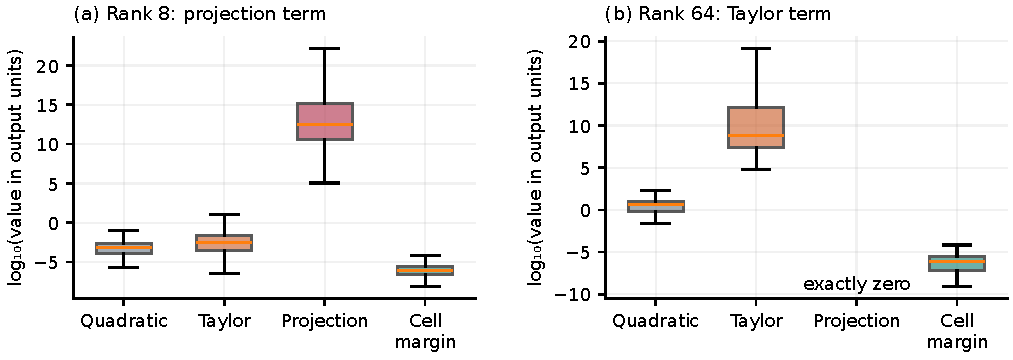
\includegraphics[width=\textwidth]{figures/model_error_budget.pdf}
  \caption{Maximum-channel omitted-quadratic, Taylor, and projection terms,
  divided by true shifted mass, compared with minimum-channel cell margins.
  These explain scales rather than additively decompose output error: mass
  uncertainty also contributes. JSON artifacts retain outliers beyond whiskers.}
  \label{fig:model-error-budget}
\end{figure*}

\subsection{GH200 Performance and Complete Costs}
\label{sec:gh200-measurements}

We measure 57 synthetic and nine trained prose trace/rank configurations on
one NVIDIA GH200. The forced PyTorch fused FlashAttention SDPA baseline
\citep{flashattention} matches BF16 inputs, scale, visible keys, and zero
dropout. Seven samples of 20 invocations provide CUDA-event and host-wall
times. Complete eager timings include screening, device decision reduction,
CPU synchronization, and output cast or actual full-batch fallback; resident
measurements exclude separately recorded setup. \Cref{sec:gh200-protocol}
gives the environment, batch semantics, and sampling details;
\cref{fig:gh200-latency} reports resident and complete-path latency.

Parallel block reduction improves the long-context, single-query resident
kernel, while small cases retain adverse results
(\cref{tab:gh200-ablation,fig:gh200-kernel-ablation}). Originally each output
coordinate occupies one thread looping serially over blocks; one query thus
exposes only 64 threads. Sharing repeated scalar arithmetic barely helps.
Assigning a CTA per coordinate exposes block parallelism, reducing the isolated
reduction from \SI{99.38}{\micro\second} to \SI{6.65}{\micro\second} at
$N=32768,Q=1$. With more queries or fewer blocks, additional CTAs and
synchronization provide less benefit and can hurt. Isolated phase measurements
diagnose this bottleneck; their sum does not replace measured complete latency
(\cref{fig:gh200-cost-breakdown}).

\begin{figure*}[!t]
  \centering
  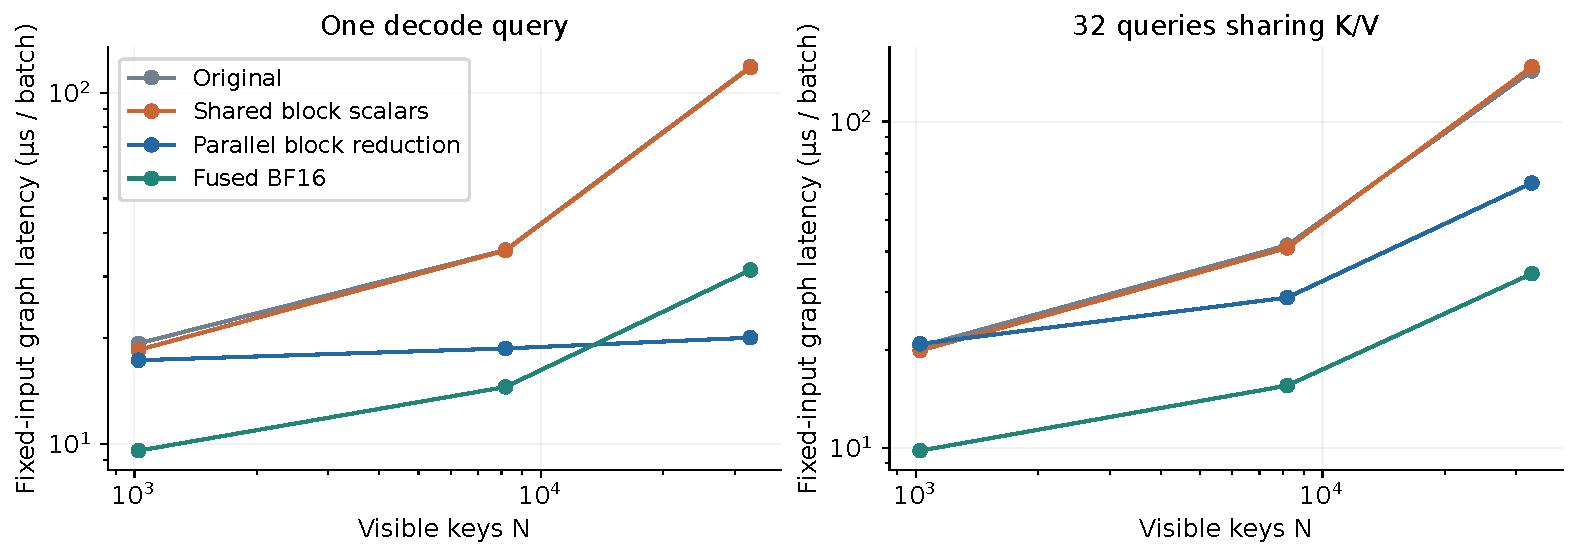
\includegraphics[width=\textwidth]{figures/gh200_kernel_ablation.pdf}
  \caption{Three CUDA implementations under matched graph replay. Sharing
  scalar work leaves serial block reduction dominant; parallelizing blocks
  helps long-context single-query inputs, with synchronization costs at small
  $N$.}
  \label{fig:gh200-kernel-ablation}
\end{figure*}

Even the favorable $N=32768,Q=1,r=4$ case loses end to end. Its resident
parallel screen takes \SI{20.09}{\micro\second} under fixed-input graph replay
versus dense attention's \SI{31.30}{\micro\second}; the complete eager path
takes \SI{83.11}{\micro\second} versus \SI{35.62}{\micro\second}, plus about
\SI{51.50}{\milli\second} of reusable summary/workspace setup. Every measured
complete path is slower than dense, so no finite reuse count repays setup
under these costs. \Cref{sec:gh200-costs} retains the footprint exclusions,
phase measurements, and amortization results.

\begin{samepage}
Across all 66 configurations, accepted numerical coordinates have zero observed
BF16 mismatches against binary64 attention but 1,691 against the fused BF16
baseline. Repeated configurations make these aggregate counts dependent.
Real-attention rounding and fused intermediate arithmetic are different
targets; the binary64 comparison is itself numerical, and the summary path is
not outward interval metadata for the directed checker.
\par
\end{samepage}


\begin{samepage}
A second run at committed implementation \texttt{d2c3668} reproduces all
66 cases with unchanged coverage and mismatch counts. Parallel-screen graph
medians change by $-1.08\%$ to $+1.42\%$, with median ratio $1.002$; every
complete path remains slower than dense. Figures and tables retain the first
sweep. \Cref{sec:gh200-reproduction} provides provenance, host-wall variation,
and the retained failed parity checks.
\par
\end{samepage}

\section{Discussion}
\label{sec:discussion}

Better certificates need information that controls the decision boundary.
Test block partitions, tighter radii, higher-order residuals, and consumer
margins separately, charging any query-dependent scan. Coupled certification
on trained traces remains unmeasured.

Faster execution needs cheaper decisions and bounded fallback work, together
with a sound GPU summary builder. The reduction ablation identifies a useful
device optimization; complete-path costs constrain its value. Our PyTorch
baseline does not exhaust Hopper and decode implementations
\citep{flashattention3,leanattention}. The contribution is a proved
real-arithmetic certificate and an empirical account of where its information
and execution costs prevent acceleration.


\clearpage
\appendix
\FloatBarrier
\section{Supporting Certificate and Moment Proofs}
\label{sec:theory-proofs}

\FloatBarrier
\subsection{Box Optimality}
\label{app:box-optimality}
\begin{proof}[Proof of \cref{thm:box-optimality}]
For the minimum, choose $m_{bj}=m^-_{bj}$ and $z_b=l_b$ if
$\nu_{bj}-c\ge0$, or $z_b=u_b$ otherwise. These simultaneous admissible
choices minimize every summand in \cref{eq:residual-identity}. Opposite mass
endpoints and $m_{bj}=m^+_{bj}$ attain the maximum. The matching inequalities
are \cref{eq:residual-enclosure}.
\end{proof}

\FloatBarrier
\subsection{The Row-Sum Quadratic Bound}
\label{app:quadratic-witness}
\begin{proof}[Proof of \cref{lem:quadratic-witness}]
The inequality $|u_a u_k|\le(u_a^2+u_k^2)/2$ and symmetry give
\begin{equation*}
 \begin{aligned}
 |u^TFu|&\le\frac12\sum_{a,k}|F_{ak}|(u_a^2+u_k^2)\\
 &=\sum_a u_a^2\sum_k|F_{ak}|\le\eta\sum_a u_a^2.
 \end{aligned}
\end{equation*}
No numerical eigendecomposition is needed.
\end{proof}

\FloatBarrier
\subsection{The Sharp Exponential Majorant}
\label{app:sharp-remainder}
\begin{proof}[Proof of \cref{lem:sharp-remainder}]
If $\rho=0$, then $t=0$. Otherwise absolute convergence of the exponential
series yields
\begin{equation*}
 \left|\sum_{n\ge3}\frac{t^n}{n!}\right|
 \le t^2\sum_{n\ge3}\frac{\rho^{n-2}}{n!}
 =\kappa(\rho)t^2.
\end{equation*}
Equality at $t=\rho>0$ forces every uniform coefficient to be at least
$\kappa(\rho)$. Substituting $n=m+3$ and using $(m+3)!\ge6m!$ gives
\begin{equation*}
 \kappa(\rho)=\sum_{m\ge0}\frac{\rho^{m+1}}{(m+3)!}
 \le\frac{\rho}{6}\sum_{m\ge0}\frac{\rho^m}{m!}.
\end{equation*}
For $\rho>0$, terms with $m\ge1$ make the inequality strict.
\end{proof}

\FloatBarrier
\subsection{Full-Score Enclosure from Signed Moments}
\label{app:full-score-enclosures}
\begin{proof}[Proof of \cref{thm:full-score-enclosures}]
Centering gives $\operatorname{mean}(t_i)=0$,
$\operatorname{mean}(t_i^2)=\sigma_b^2$, and
$\operatorname{mean}(x_{ij})=0$. Writing
$r_i=e^{t_i}-1-t_i-t_i^2/2$, \cref{lem:sharp-remainder} gives
$\operatorname{mean}|r_i|\le\tau_b$. Thus the projected mass lies in
$w_b[A_b-\tau_b,A_b+\tau_b]$. Jensen's inequality also bounds it below by
$w_b$, proving \cref{eq:projected-mass}.

The projected centered numerator equals
\begin{equation*}
 w_b\left[(C_b^Tu)_j+\tfrac12u^TH_{bj}u+
 \operatorname{mean}(r_i x_{ij})\right].
\end{equation*}
Apply \cref{lem:quadratic-witness} to $H_{bj}-D_{bj}$ and use
$|\operatorname{mean}(r_i x_{ij})|\le\tau_bR_{bj}$ to obtain
\cref{eq:projected-numerator}.

Restoring discarded coordinates multiplies each positive projected weight by
$e^{e_i}\in[e^{-\epsilon_b},e^{\epsilon_b}]$, proving \cref{eq:full-mass}.
Since $|e^{e_i}-1|\le e^{\epsilon_b}-1$, the centered numerator changes by
at most
\begin{equation*}
 \begin{aligned}
 &(e^{\epsilon_b}-1)R_{bj}\sum_{i\in b}e^{a_b-s+t_i}\\
 &\qquad\le(e^{\epsilon_b}-1)\widetilde u_bR_{bj}.
 \end{aligned}
\end{equation*}
Adding this perturbation proves \cref{eq:full-numerator}.
\end{proof}

\FloatBarrier
\subsection{Exact Polygon Support}
\label{app:polygon-support}
The rational optimizer enumerates polygon vertices. Candidate masses are
$l_b,u_b$ and $m^-_{bj}/s,m^+_{bj}/s$ for each nonzero
$s\in\{p_{bj},q_{bj}\}$. At a feasible mass $z$, the centered endpoints are
$\max(m^-_{bj},p_{bj}z)$ and $\min(m^+_{bj},q_{bj}z)$.
These cover intersections of vertical, horizontal, and sloping boundaries.
Distinct sloping lines meet at $z=0$, necessarily a mass endpoint if feasible
under $l_b\ge0$; coincident lines and degenerate segments add no candidates.
A linear objective attains its extrema at these vertices. Empty candidate
sets indicate inconsistent metadata and are rejected. The number of rational
operations is constant per block/channel; their bit cost is not.

\FloatBarrier
\subsection{Boundary Geometry}
\label{app:boundary-geometry}
\begin{example}\label{ex:boundary-geometry}
Two blocks with centers $0,2$, masses in $[1,2]$, and zero centered numerators
have output range $[2/3,4/3]$. Boundary signs certify $(0.6,1.4)$. A symmetric
residual bound about $1$ using midpoint masses has radius $0.5$ and fails.
This is a strict improvement in this example, not a dominance claim over
every correlated certificate.
\end{example}

\begin{figure}[!htbp]
 \centering
 % Native vector fragment. Required: tikz; arrows.meta; cmk{blue,orange,green,gray}.
% Exact witness: nu=(0,2), z_1,z_2 in [1,2], m_1=m_2=0.
% On 1/4 <= c <= 7/4, L(c)=2-3c and U(c)=4-3c.
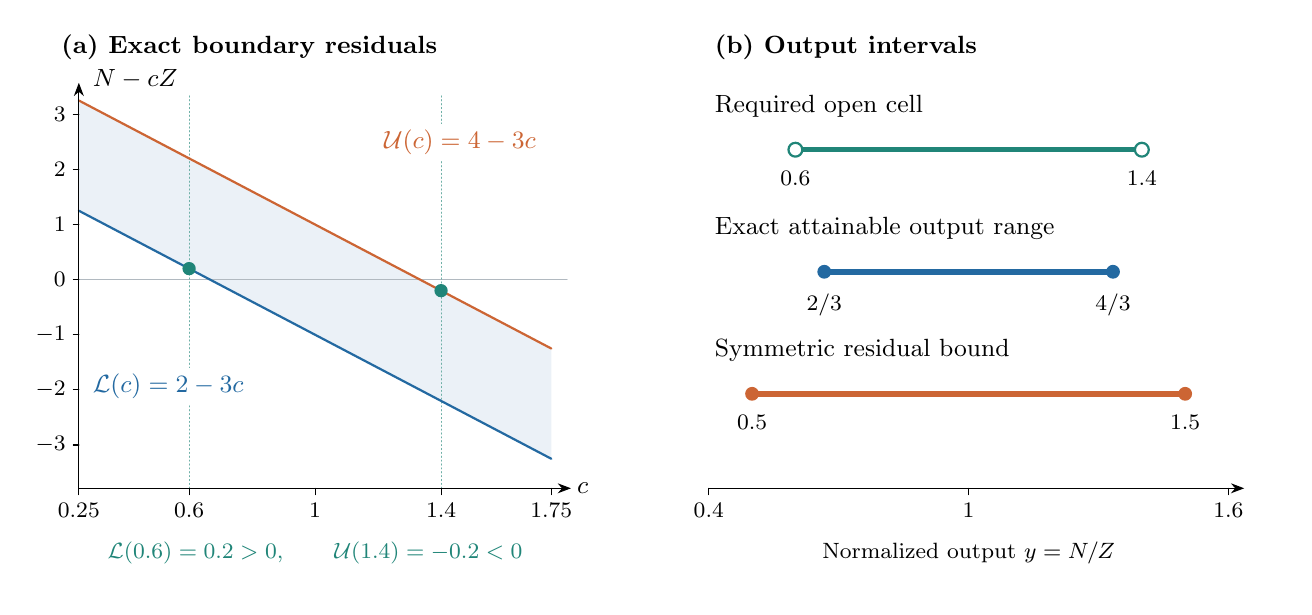
\begin{tikzpicture}[font=\small, line cap=round, line join=round,
  >=Stealth, every node/.style={inner sep=2pt}]
  \path[use as bounding box] (-0.65,-0.9) rectangle (15.3,6.2);
  \node[anchor=west,font=\small\bfseries] at (-0.3,5.95)
    {(a) Exact boundary residuals};
  % x = 4(c-1/4); y = 3 + 0.7 residual.
  \fill[cmkblue!9] (0,3.875)--(6,0.725)--(6,2.125)--(0,5.275)--cycle;
  \draw[cmkgray!55,thin] (0,3)--(6.2,3);
  \draw[cmkgreen!65,densely dotted] (1.4,0.35)--(1.4,5.35);
  \draw[cmkgreen!65,densely dotted] (4.6,0.35)--(4.6,5.35);
  \draw[cmkblue,thick] (0,3.875)--(6,0.725);
  \draw[cmkorange,thick] (0,5.275)--(6,2.125);
  \node[anchor=west,text=cmkorange,fill=white] at (3.8,4.75)
    {$\mathcal U(c)=4-3c$};
  \node[anchor=west,text=cmkblue,fill=white] at (0.1,1.65)
    {$\mathcal L(c)=2-3c$};
  \fill[cmkgreen] (1.4,3.14) circle (2.4pt);
  \fill[cmkgreen] (4.6,2.86) circle (2.4pt);
  \draw[->] (0,0.35)--(6.25,0.35) node[anchor=west] {$c$};
  \draw[->] (0,0.35)--(0,5.5);
  \node[anchor=south west] at (0.1,5.35) {$N-cZ$};
  \foreach \x/\lab in {0/0.25,1.4/0.6,3/1,4.6/1.4,6/1.75} {
    \draw (\x,0.35)--(\x,0.27);
    \node[anchor=north,font=\footnotesize] at (\x,0.24) {$\lab$};
  }
  \foreach \y/\lab in {0.9/-3,1.6/-2,2.3/-1,3/0,3.7/1,4.4/2,5.1/3} {
    \draw (0,\y)--(-0.07,\y);
    \node[anchor=east,font=\footnotesize] at (-0.09,\y) {$\lab$};
  }
  \node[anchor=north,align=center,text=cmkgreen,font=\footnotesize]
    at (3,-0.25)
    {$\mathcal L(0.6)=0.2>0,\qquad\mathcal U(1.4)=-0.2<0$};
  \begin{scope}[xshift=8cm]
    \node[anchor=west,font=\small\bfseries] at (0,5.95)
      {(b) Output intervals};
    % x = 5.5(y-0.4); each row has its own descriptive label.
    \node[anchor=west] at (0,5.2) {Required open cell};
    \draw[cmkgreen,line width=2pt] (1.1,4.65)--(5.5,4.65);
    \foreach \x/\lab in {1.1/0.6,5.5/1.4} {
      \draw[cmkgreen,fill=white,thick] (\x,4.65) circle (2.5pt);
      \node[anchor=north,font=\footnotesize] at (\x,4.45) {$\lab$};
    }
    \node[anchor=west] at (0,3.65) {Exact attainable output range};
    \draw[cmkblue,line width=2pt] ({5.5*(2/3-0.4)},3.1)--({5.5*(4/3-0.4)},3.1);
    \foreach \x/\lab in {{5.5*(2/3-0.4)}/{2/3},{5.5*(4/3-0.4)}/{4/3}} {
      \fill[cmkblue] ({\x},3.1) circle (2.5pt);
      \node[anchor=north,font=\footnotesize] at ({\x},2.9) {$\lab$};
    }
    \node[anchor=west] at (0,2.1) {Symmetric residual bound};
    \draw[cmkorange,line width=2pt] (0.55,1.55)--(6.05,1.55);
    \foreach \x/\lab in {0.55/0.5,6.05/1.5} {
      \fill[cmkorange] (\x,1.55) circle (2.5pt);
      \node[anchor=north,font=\footnotesize] at (\x,1.35) {$\lab$};
    }
    \draw[->] (0,0.35)--(6.8,0.35);
    \foreach \x/\lab in {0/0.4,3.3/1,6.6/1.6} {
      \draw (\x,0.35)--(\x,0.27);
      \node[anchor=north,font=\footnotesize] at (\x,0.24) {$\lab$};
    }
    \node[anchor=north,font=\footnotesize] at (3.3,-0.25)
      {Normalized output $y=N/Z$};
  \end{scope}
\end{tikzpicture}

 \caption{Boundary residuals for \cref{ex:boundary-geometry}. The attained
 output range is closed; the certified open cell is illustrative, not a BF16
 rounding cell.}
 \label{fig:boundary-geometry}
\end{figure}

\FloatBarrier
\subsection{Joint Value Coupling}
\label{app:joint-coupling}
\begin{example}\label{ex:joint-coupling}
For $z\in[1,4]$, $m\in[1/2,3/2]$, and $-z/2\le m\le z/2$, consider
$m-z/4$. The box gives $[-1/2,5/4]$; the cone with the mass interval gives
$[-3,1]$. Intersecting these scalar bounds gives $[-1/2,1]$, whereas joint
optimization gives $[-1/2,3/4]$. This compares metadata geometry without
asserting token realizability of every vertex.
\end{example}

\FloatBarrier
\subsection{Margin and Refinement}
\label{app:margin-refinement}
The residual width separates mass and numerator uncertainty:
\begin{equation}
 \begin{aligned}
 W_j(c)&=\mathcal U_j(c)-\mathcal L_j(c)\\
 &=\sum_b\bigl[m^+_{bj}-m^-_{bj}+|\nu_{bj}-c|(u_b-l_b)\bigr].
 \end{aligned}
 \label{eq:residual-width}
\end{equation}
\begin{samepage}
\begin{proposition}[Margin versus uncertainty]\label{prop:margin-uncertainty}
For $a_j<y_j<b_j$, certification follows if
\begin{equation*}
 \begin{aligned}
 W_j(a_j)&<Z(y_j-a_j),\\
 W_j(b_j)&<Z(b_j-y_j).
 \end{aligned}
\end{equation*}
\end{proposition}
\end{samepage}
\begin{proof}
The lower endpoint is at least the true residual minus its enclosure width;
the upper endpoint is at most the true residual plus its width. The proposed
inequalities therefore give both strict signs.
\end{proof}
This explanatory condition requires unknown truth, so is not an executable
test. It explains difficult near-midpoint coordinates and prioritizing large
width contributions. If sound widths converge to zero and the output stays
strictly inside a fixed cell, that cell eventually passes. The bounded executor
does not assume convergence before fallback.

\FloatBarrier
\subsection{Diagonal Retention Need Not Produce Nested Intervals}
\label{app:diagonal-nonnesting}
Retaining the diagonal weakly reduces the row-sum witness but shifts the
approximation center, so the resulting intervals need not be nested.
For $H_{11}=9$, $H_{23}=H_{32}=10$, all other entries zero, and $u=(1,0,0)$,
both witnesses equal $10$. Retaining the diagonal changes $[-10,10]$ to
$9+[-10,10]$. Acceptance need not improve for every cell; both representations
are exposed by the implementation.

\FloatBarrier
\subsection{Remainder and Projection Growth}
\label{app:remainder-growth}
\Cref{fig:remainder-mechanism} compares the sharp remainder coefficient with
the Lagrange bound and isolates the separate cost of discarded-score variation.
\begin{figure}[!htbp]
 \centering
 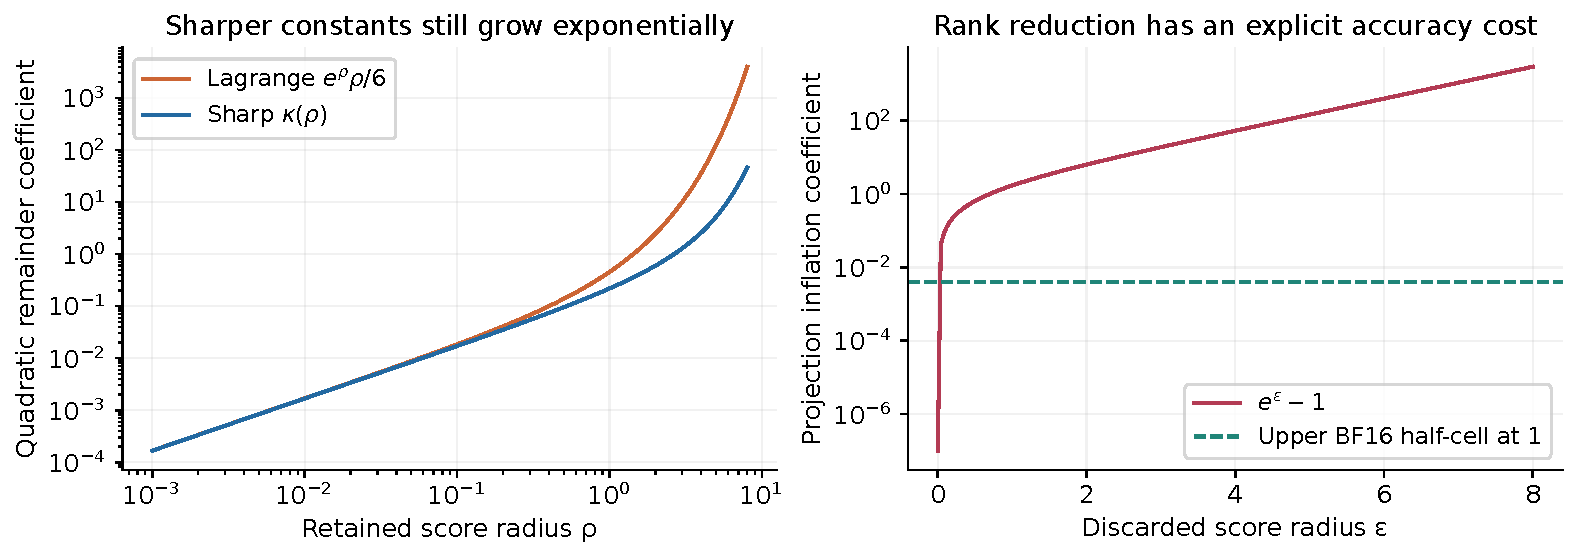
\includegraphics[width=\textwidth]{figures/remainder_mechanism.pdf}
 \caption{The sharp coefficient improves the Lagrange constant but still
 grows exponentially. Discarded scores impose a separate exponential cost.
 The BF16 line is a unit-scale guide, not a sufficient certificate.}
 \label{fig:remainder-mechanism}
\end{figure}

\FloatBarrier

\section{Formalization and General Consumers}
\label{app:formalization}

Lean 4.24.0 and the pinned mathlib revision build all 64 local theorems.
The complete axiom audit contains only \code{propext}, \code{Classical.choice},
and \code{Quot.sound}. The \artifact{results/lean-verification.json}{audit manifest}
records source hashes and dependencies for every declaration; the
\artifact{docs/FORMALIZATION.md}{formalization map} gives the complete list.

\paragraph{The composed theorem.}
The observation theorem in \cref{tab:formalization} applies derived block bounds
to the actual finite, per-token real exponential quotient. Its witness assumes
nonempty tokens, centering, nonnegative radii, radius bounds, retained-tensor
symmetry, and an absolute row-sum bound on the omitted signed tensor.
It does not assume the Taylor remainder or the final enclosure.
Lean uses finite sums where the manuscript
uses means: for a block of size $n$, its $H$, $D$, and $\eta$ are multiplied by $n$.

\begin{table*}[t]
\centering
\caption{Key declarations in the built Lean proof chain. The complete audit covers 64 theorems.}
\label{tab:formalization}
\begin{tabularx}{\textwidth}{@{}lX@{}}
\toprule
Declaration & Established property \\
\midrule
\code{exp_remainder_sharp} & Actual exponential-series remainder bound. \\
\code{quadratic_rowsum_bound} & Symmetric omitted-tensor bound from absolute row sums. \\
\code{finite_mean_centering} & Exact means supply finite-sum centering. \\
\code{second_moment_contraction} & Projected second-moment contraction. \\
\code{signed_moment_contraction} & Signed key/value tensor contraction. \\
\code{full_score_enclosure} & Full-score block mass and centered-numerator bounds. \\
\code{full_attention_observation} & Strict cell membership for the real exponential quotient. \\
\code{observation_cell_iff} & Necessary-and-sufficient strict signs over the independent box. \\
\code{centered_value_mass_coupling} & Positive-weight value-range/mass dependence. \\
\bottomrule
\end{tabularx}
\end{table*}

\paragraph{Executable bridges.}
The rational exponential, interval conversion, BF16 cell construction,
polygon support optimizer, and runtime identity validation are not extracted
from Lean. Neither are CUDA memory accesses, instruction rounding, overflow,
compiler transformations, or state updates. The concrete IEEE model, including
signed zero, infinities, NaNs, and midpoint ties, is not formalized.
\code{monotone_rounding} assumes an abstract monotone real function.
The numerical summary path cannot discharge the directed checker's sound-input
premise. These are implementation obligations beyond the real theorem.

\subsection{Other Observation Contracts}
If a consumer is constant on a set containing the output, its value is fixed
(\code{constant_consumer}). For monotone rounding $Q$,
$l\leq y\leq u$ and $Q(l)=Q(u)$ suffice. For argmax, $l_w>u_j$ for all $j\ne w$
certifies winner $w$ (\code{strict_argmax}). Equality of complete deterministic
state transitions implies equality of repeated execution
(\code{transition_composition}); this theorem does not prove an executor's
transition-equality premise.

\subsection{Smooth Gates}
The residual certificate applies to any positive normalized weights with
sound block envelopes. Signed unnormalized contractions instead sum intervals.
For a smooth gate, let
$p=\phi(t+\alpha)$, $p_0=\phi(t)$, and $p_1=\phi'(t)$. Then
\begin{align}
 &p(s+\gamma)-(p_0s+p_1\alpha s+p_0\gamma)\nonumber\\
 &\qquad=p_1\alpha\gamma+(p-p_0-p_1\alpha)(s+\gamma).
 \label{eq:gate-identity}
\end{align}
If $|\alpha|\leq\rho_g$, $|\gamma|\leq\rho_u$, and
$|p-p_0-p_1\alpha|\leq M\rho_g^2/2$, then
\begin{equation}
 |\mathrm{error}|\leq |p_1|\rho_g\rho_u
       +\tfrac12M\rho_g^2(|s|+\rho_u).
\end{equation}
Lean proves \code{gated_residual_identity} and \code{gated_remainder_bound}.
A curvature witness for a concrete gate remains a separate obligation.
For SwiGLU, absolute downstream weights multiply these nonnegative radii
before summation. Contracted coefficients may save an intermediate while
requiring more storage than the original weights; no feed-forward speedup
is established here.

\FloatBarrier
\section{Validation and Experimental Protocols}
\label{sec:experiments-appendix}

\FloatBarrier
\subsection{Arithmetic and Implementation Validation}
\label{sec:experimental-validation}

The successful Lean 4.24.0 build and axiom audit cover 64 local declarations,
including the exponential remainder, finite signed tensor contractions,
full-score block enclosure, and composed real-attention quotient. The only
axioms are \texttt{propext}, \texttt{Classical.choice}, and \texttt{Quot.sound};
\artifact{results/lean-verification.json}{Lean audit manifest} records source hashes and per-theorem
dependencies. The polygon optimizer, rational exponential routine, BF16 cell
constructor, state identity, and CUDA instruction semantics remain separate
implementation obligations.

The 46-test CPU suite includes randomized enclosure tests, 500 exact polygon
comparisons with an independent half-plane intersection implementation,
40 direct 100-digit attention comparisons across rank and refinement, and
40 numerical/exact geometry comparisons. Invalid dimensions, nonintegral
indices, negative bounds, unsupported domains, stale source/query/shift state,
and midpoint behavior are covered.

\begin{samepage}
This audit found an arithmetic defect:
integer endpoints allowed reciprocal evaluation through Python's floating-point
\mbox{\texttt{1 / int}}, so the upper endpoint of $[1,1]/[3,3]$ could lie below $1/3$.
Endpoints and scale factors now normalize to exact fractions; the regression
requires both endpoints to equal $1/3$ exactly.
\end{samepage}

The imported CUDA checker retains all 74 rational-certified rows among
160 rationally generated rows, certifies no rationally refused row in that
fixture, and rejects 13 invalid-domain or strict-boundary controls. Numerical
fixtures compare the original, shared-scalar, and parallel implementations and
dense block correction against CPU results. Memory, race, and synchronization
checks report no errors on the exercised numerical paths; imported CUDA memory
checking also reports no errors. These finite checks complement the theorem
chain without establishing instruction-level correctness for all inputs.

\FloatBarrier
\subsection{Exact-Rational Coupling Checks}
\label{sec:coupling-validation}

Independent high-precision coverage comparisons use 110 decimal digits and a
scaled $10^{-95}$ tolerance to compare against exact zero-width intervals.
An initial zero-tolerance attempt failed through cancellation in a constant
channel and is documented. Certificate and rational-oracle comparisons use
exact fractions without this tolerance. Stored decimal endpoints are display
approximations; broad-channel failures and exact-midpoint abstentions remain
in the artifact.

\begin{table}[!htbp]
  \centering
  \caption{Initial exact-rational coupling results. Denominators count
  coordinates, not independent model examples.}
  \label{tab:coupling-results}
  \begin{tabular}{lr}
    \toprule
    Result & Count \\
    \midrule
    Box certificate accepts & $57/149$ \\
    Coupled certificate accepts & $61/149$ \\
    Global hull accepts & $50/149$ \\
    Narrower coupled residual & $30/149$ \\
    Unchanged residual width & $119/149$ \\
    Accepts beyond global hull & $1$ \\
    False certificate / coverage failure & $0$ \\
    \bottomrule
  \end{tabular}
\end{table}

\FloatBarrier
\subsection{Uncertainty Localization and GPU Controls}
\label{sec:localized-uncertainty}

The CPU experiment in \cref{sec:coupling-experiment} isolates correction work.
\Cref{fig:selective-refinement} shows the selected token fractions for every
query before the GPU controls below compare complete-output coverage and cost.

\begin{figure}[!htbp]
  \centering
  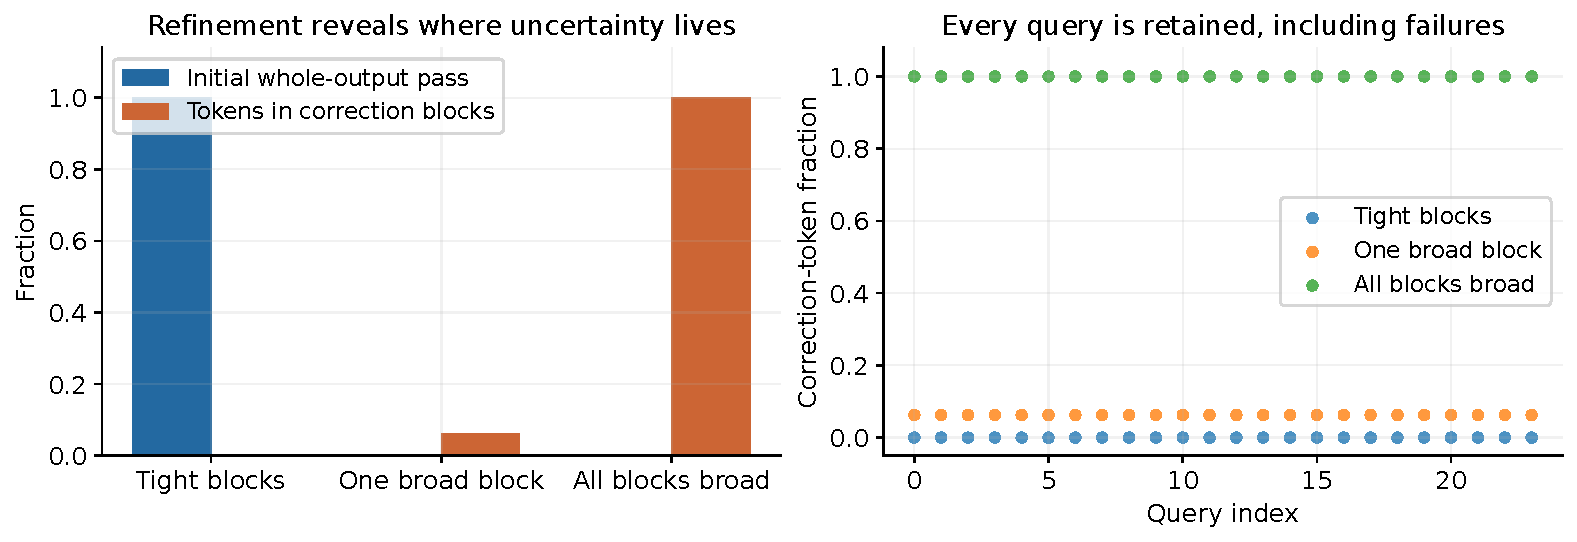
\includegraphics[width=\textwidth]{figures/selective_refinement.pdf}
  \caption{Correction-token fractions for every query in tight, mixed, and
  broad CPU inputs. Local uncertainty permits local correction; diffuse
  uncertainty requires all tokens. Full-source validation reads are additional
  and included in CPU timings.}
  \label{fig:selective-refinement}
\end{figure}

GPU synthetic controls use $d=h=64$ and BF16 input values represented exactly
in binary64 on the summary path. Tight clusters can pass completely. Moderate
cases pass 10,197 of 19,008 coordinates across configurations but none of
297 complete outputs; these aggregates reuse seeded inputs across ranks.
The centered-value control passes 1,986 of 2,048 coordinates but only 6 of
32 outputs. Complete-output acceptance is a conjunction of coordinate
decisions, so high marginal coverage need not yield useful output coverage.
This observation assumes no coordinate independence. Exact-midpoint controls
reject every strict cell by design. In the measured GPU path, one failed
coordinate triggers full-batch fallback (\cref{fig:gh200-coverage-cost}).

\begin{figure}[!htbp]
  \centering
  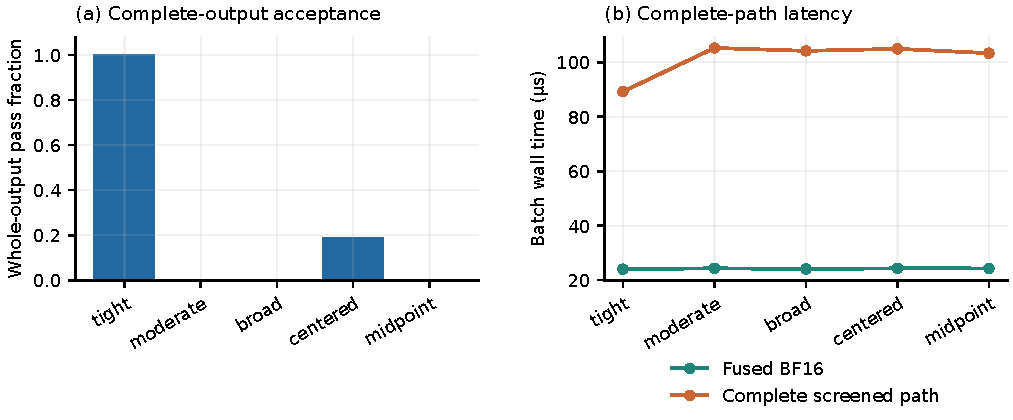
\includegraphics[width=\textwidth]{figures/gh200_coverage_cost.pdf}
  \caption{Whole-output coverage and complete GPU costs for rank-four,
  $N=8192$, $Q=32$ controls varying uncertainty and cell margins. The cost
  includes the full-batch fallback triggered by any failed coordinate.}
  \label{fig:gh200-coverage-cost}
\end{figure}

\FloatBarrier
\subsection{Trained-Activation Capture and Diagnostics}
\label{sec:trained-protocol}

No coordinate or whole output passes the numerical screen on either trained
activation set. Rank eight covers all 24 layers and 14 query heads over six
prefixes: 2,016 head instances and 129,024 coordinates. Full rank covers layers
0, 12, and 23, adding 252 head instances. We capture actual post-RoPE Q/K/V
arguments at the attention call of Qwen2.5-0.5B \citep{qwen25}, pinned revision
\texttt{060db64} (the full commit hash is recorded in the
\artifact{results/model_traces/manifest.json}{capture manifest}), using
Transformers 4.51.3
and BF16 weights. Three deterministic original texts cover prose, code, and
arithmetic at prefix lengths 1,024 and 4,096. The final prefill query sees the
entire prefix; contiguous GQA groups contain seven query heads per KV head,
and scaling by $1/8$ is exact. This is an activation diagnostic, not a
language-model accuracy benchmark or production-traffic sample.

\begin{table}[!htbp]
  \centering
  \caption{Medians of trained-activation radius and cell-margin diagnostics.
  Full rank uses the three representative layers.}
  \label{tab:trained-radii}
  \begin{tabular}{lrr}
    \toprule
    Diagnostic & Rank 8 & Rank 64 \\
    \midrule
    Maximum-block retained bound $\rho$ & 1.32 & 29.91 \\
    Maximum-block discarded bound $\epsilon$ & 34.24 & 0 \\
    Actual maximum projected score deviation & 0.85 & 8.91 \\
    Minimum-channel BF16 boundary margin
      & $8.95\times10^{-7}$ & $6.66\times10^{-7}$ \\
    \bottomrule
  \end{tabular}
\end{table}

\begin{figure}[!htbp]
  \centering
  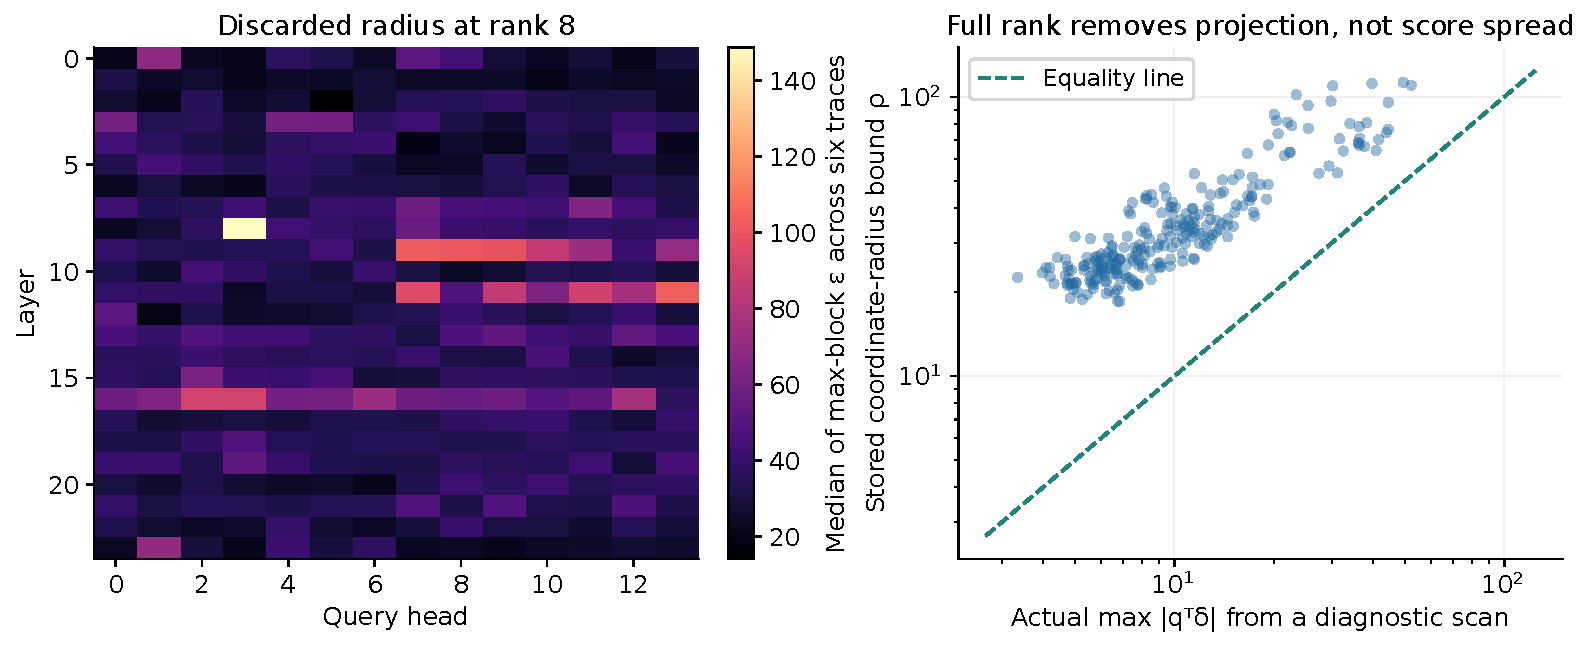
\includegraphics[width=\textwidth]{figures/model_score_radii.pdf}
  \caption{Trained-model score radii by layer and head. Low rank leaves large
  discarded-score variation; full-rank coordinate bounds exceed scan-derived
  radii, while actual score variation remains substantial. Computing scanned
  diagnostic radii reads tokens and is not free query metadata.}
  \label{fig:model-score-radii}
\end{figure}

\FloatBarrier
\subsection{GH200 Environment and Timing Protocol}
\label{sec:gh200-protocol}

The final sweep contains 57 synthetic and nine actual prose trace/rank
configurations on one NVIDIA GH200: compute capability 9.0, 97,871 MiB reported
GPU memory, driver 580.105.08, CUDA 12.8, and PyTorch 2.7.0. Synthetic cases vary
$N\in\{1024,8192,32768\}$, rank, spread, and $Q\in\{1,32\}$. Here $Q=32$
is a noncausal query batch sharing K/V, not independent serving requests.
Trace cases use seven query heads sharing one KV head at the final prefix.

The baseline explicitly forces PyTorch's fused FlashAttention SDPA backend
\citep{flashattention}, matching BF16 input values, scale, visible keys, and
zero dropout. A separate binary64 softmax/matmul computation checks outputs.
Seven samples of 20 invocations provide raw CUDA-event and host-wall times;
plotted quantiles summarize those samples, not workload confidence intervals.
Resident timings exclude setup; construction, uploads, casts, allocations,
workspace, and graph capture are recorded separately. Complete eager timings
include screening, device decision reduction, CPU synchronization, and either
an output cast or executed full-batch fallback (\cref{fig:gh200-latency}).

\begin{figure}[!htbp]
  \centering
  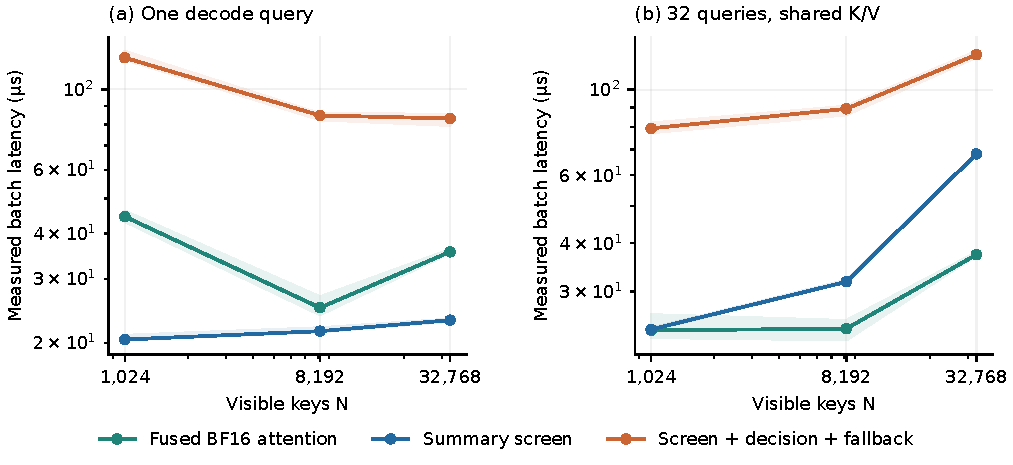
\includegraphics[width=\textwidth]{figures/gh200_latency.pdf}
  \caption{GH200 resident screening and complete-path latency against fused
  dense attention for tight rank-four inputs. Wall-clock medians and
  10th--90th sample quantiles include each complete path's actual decisions
  and fallback behavior.}
  \label{fig:gh200-latency}
\end{figure}

The eager timing helper performs three warmup calls and synchronizes before
sampling. Each sample brackets 20 invocations with CUDA events, waits for the
ending event, and divides both event elapsed time and host-wall elapsed time
by 20. Host samples therefore include Python launch and synchronization
costs. Graph measurements first warm the operation on a separate stream,
capture 20 invocations with fixed inputs, then warm graph replay three times
and collect seven replay samples. Reported replay times are divided by 20;
graph capture time is stored separately. No adaptive scheduler or fallback is
captured in the replay graph.

All 66 recorded cases use seed 902105. The 57 synthetic configurations contain
19 tight, 18 moderate, 18 broad, one centered-value, and one exact-midpoint
case. Seeded input generation is repeated across retained ranks, so aggregate
acceptance counts reuse inputs. The nine GPU trace cases are three prose
captures, from layers 0, 12, and 23 at prefix length 4,096, evaluated at ranks
0, 4, and 16. They are separate from the rank-eight and full-rank CPU activation
diagnostics.

\FloatBarrier
\subsection{Kernel Ablation, Setup, and Footprint}
\label{sec:gh200-costs}

Even the favorable $N=32768,Q=1,r=4$ case loses end to end. Its resident
parallel screen takes \SI{20.09}{\micro\second} under fixed-input graph replay
versus dense attention's \SI{31.30}{\micro\second}; the complete eager path
takes \SI{83.11}{\micro\second} versus \SI{35.62}{\micro\second}, plus about
\SI{51.50}{\milli\second} of reusable summary/workspace setup. CPU
moment-and-extrema arrays occupy 1,000,448 bytes, the uploaded box summary
869,376 bytes, and original BF16 K/V 8,388,608 bytes. These payloads exclude
262,144 bytes of group indices and Python object/hash overhead; scratch and
retained original K/V are reported separately. Neither serving-system memory
savings nor a complete-path speedup follows. Every measured complete path is
slower than dense, so no finite reuse count repays setup under these costs
(\cref{fig:gh200-amortization}).

\begin{table}[!htbp]
  \centering
  \caption{Matched graph replay medians in microseconds for tight rank-four
  inputs. All three screening implementations and the dense baseline are
  retained, including the adverse small-input case.}
  \label{tab:gh200-ablation}
  \begin{tabular}{rrrrrr}
    \toprule
    $N$ & $Q$ & Original & Shared scalar & Parallel & Dense \\
    \midrule
    1024 & 32 & 20.47 & 19.87 & 20.84 & 9.80 \\
    8192 & 1 & 35.69 & 35.60 & 18.72 & 14.55 \\
    32768 & 1 & 118.65 & 118.14 & 20.09 & 31.30 \\
    32768 & 32 & 143.28 & 147.52 & 64.89 & 34.21 \\
    \bottomrule
  \end{tabular}
\end{table}

\begin{figure}[H]
  \centering
  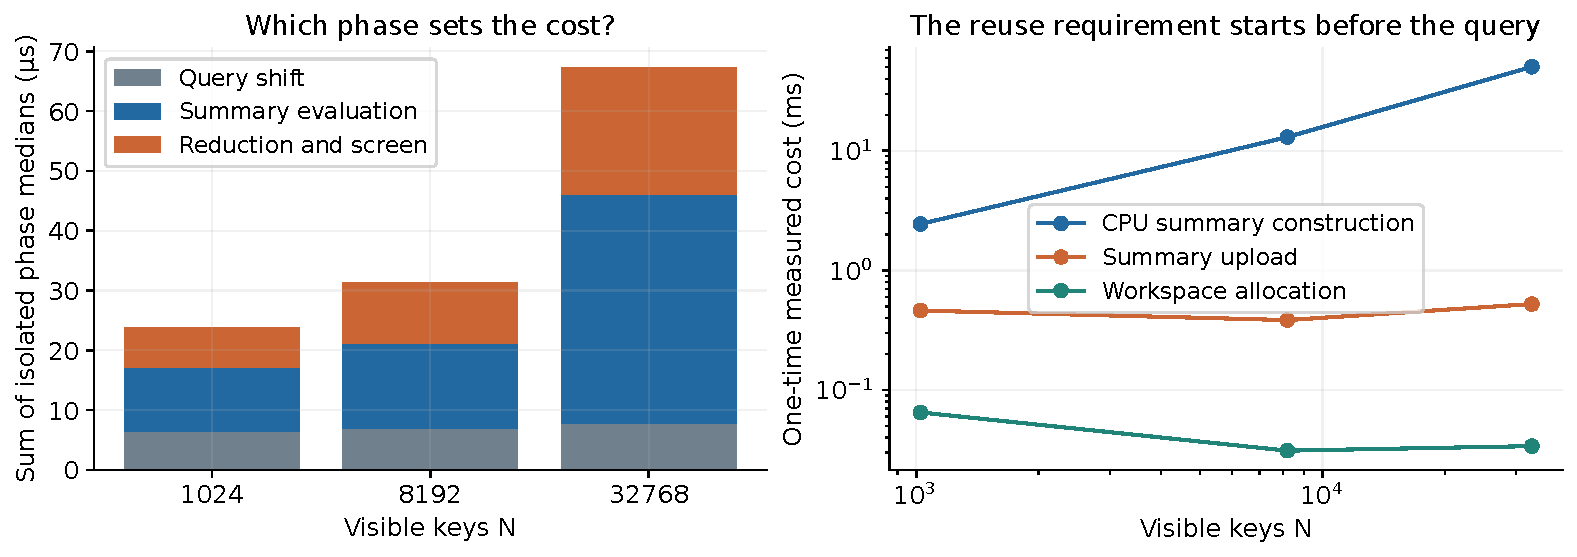
\includegraphics[width=\textwidth]{figures/gh200_cost_breakdown.pdf}
  \caption{Isolated GPU phase medians and summary setup costs. CPU
  construction, upload, and workspace allocation remain explicit; complete
  latency is measured separately rather than reconstructed from phase sums.}
  \label{fig:gh200-cost-breakdown}
\end{figure}

\begin{figure}[H]
  \centering
  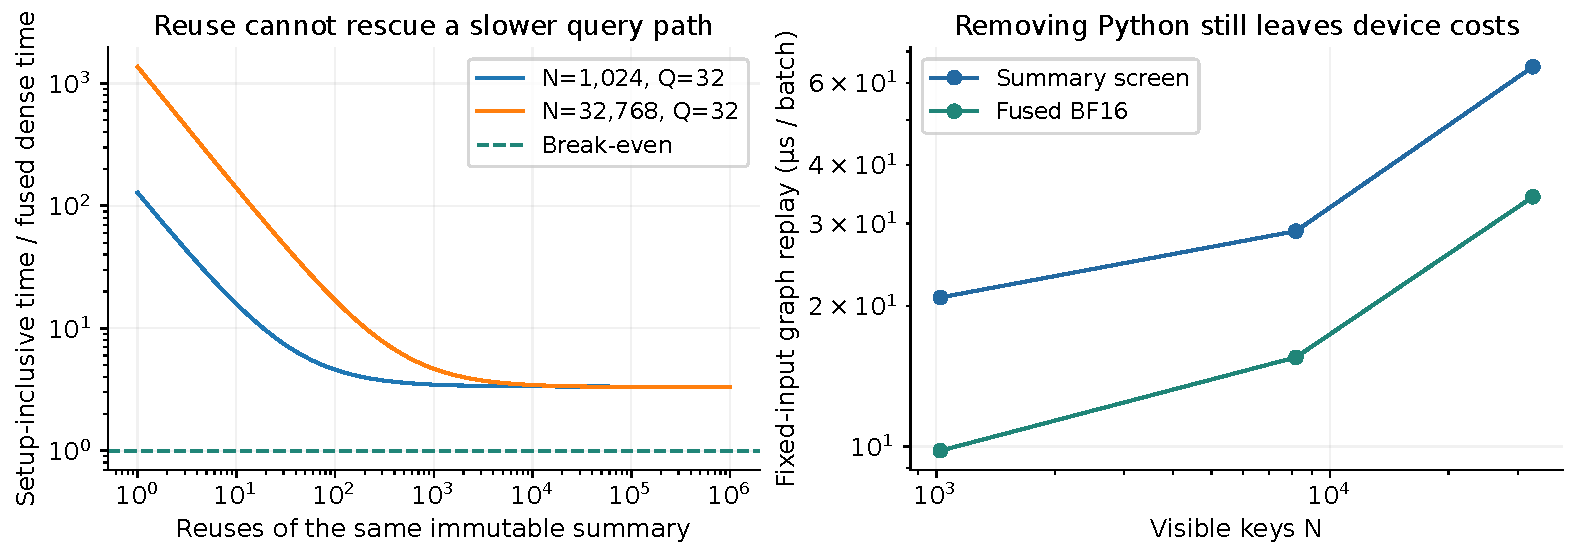
\includegraphics[width=\textwidth]{figures/gh200_amortization.pdf}
  \caption{Setup amortization and matched graph device costs. No measured
  complete path has a finite setup break-even. Fixed-input graph replay omits
  the adaptive host decision and constitutes a separate experiment.}
  \label{fig:gh200-amortization}
\end{figure}

\begin{minipage}{\textwidth}
\subsection{Retained Failures and Same-Machine Reproduction}
\label{sec:gh200-reproduction}

The first trained-trace parity attempt failed nine absolute-residual tolerance
checks because broad bounds had extremely large magnitudes. A scaled
$10^{-12}$ comparison addresses this diagnostic scaling while still requiring
identical screen decisions and independent output checks; the maximum observed
scaled variant difference is $1.33\times10^{-15}$. The nine failures and original
scalar-only sweep are preserved. This tolerance changes implementation-parity
diagnostics, not certificate bounds.

Figures and tables retain the first complete sweep. A second GH200 run measures
commit \texttt{d2c3668}, including final host ABI guards and formatted sources.
\artifact{results/gh200/provenance.json}{GH200 provenance manifest} records source, library, and trace hashes;
both original and reproduction measurements remain available. All 66 cases
pass validation again with unchanged coverage and mismatch counts. Parallel
screen graph medians change by $-1.08\%$ to $+1.42\%$ across cases, with median
ratio $1.002$. Complete-path and dense host-wall medians are noisier, with
median ratios $1.075$ and $1.112$. Every complete screened path remains slower
than dense, with no finite setup break-even. This reproduces the conclusions
on the same machine, without estimating variation across devices, model
families, or serving systems.
\par
\end{minipage}

\FloatBarrier


\clearpage
\bibliographystyle{icml2026}
\bibliography{references}
\end{document}
